\documentclass[../main.tex]{subfiles}
\graphicspath{{\subfix{../images/}}}
\begin{document}

        
        The limbic system \index{limbic system} is a collection of complicated structures in the center of the brain, which surround the brain stem like a border (Latin: limbus).
        The limbic system is the \emph{control center of the endocrine\footnote{endocrine: related to the inner secretion of glands}, vegetative\footnote{vegetative: Not subject to conscious control}and mental regulation systems.}
        It processes stimuli from the interior (endogenous) and the exterior of the body (exogenous).
        The limbic system controls the emotional behavior and is the center of feelings.
        
        %Blausen.com staff (2014). "Medical gallery of Blausen Medical 2014". WikiJournal of Medicine 1 (2). DOI:10.15347/wjm/2014.010. ISSN 2002-4436.

        \begin{figure}[htp]
        \centering
         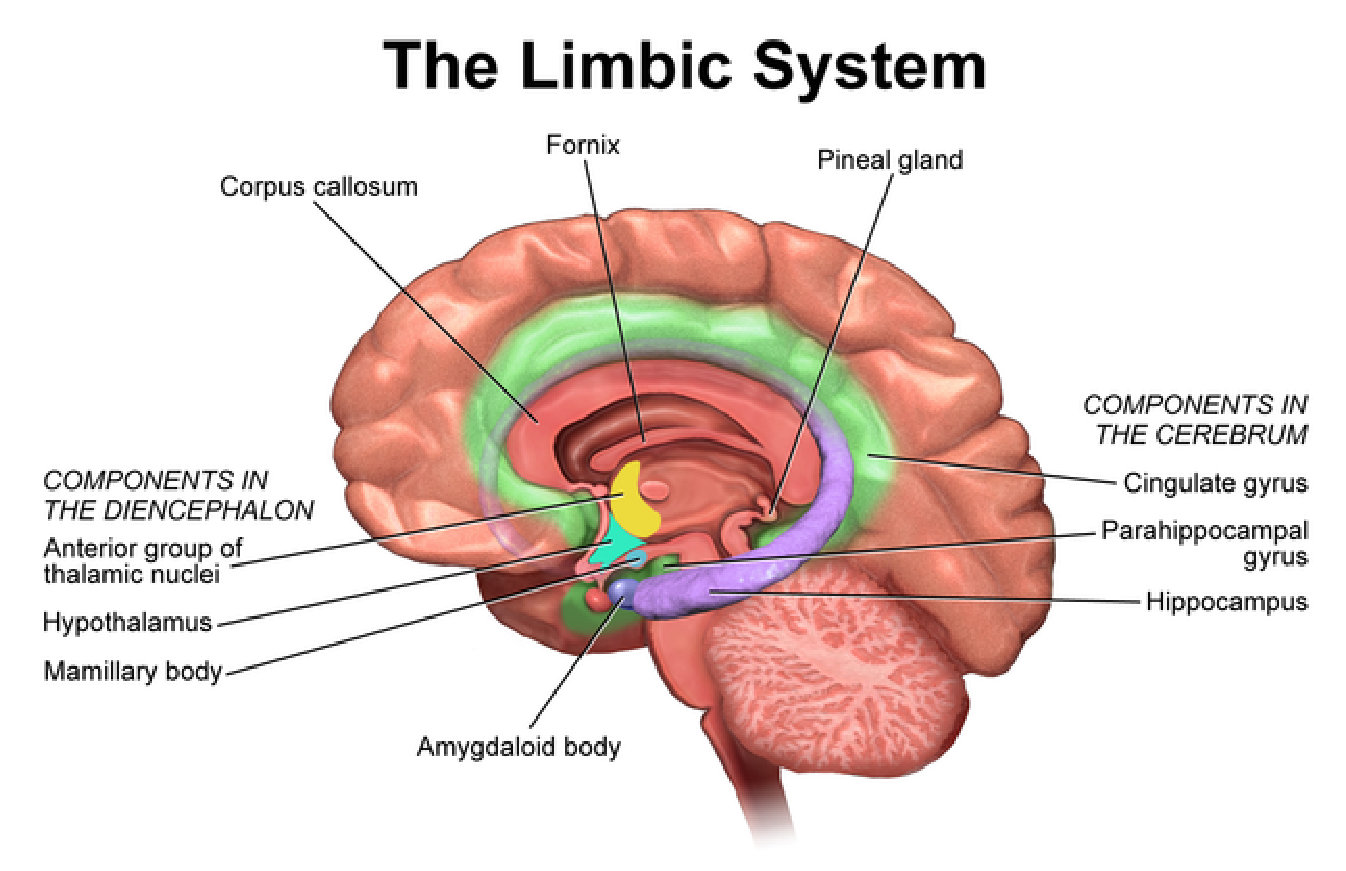
\includegraphics[width=12cm]{LimbicSystem.eps}
          \caption{Diagram of the limbic system~\cite{BlausenLimbic}}
        \end{figure}

        Stress starts already at the sensory organs. An impulse is perceived and it causes in the nerve cells electric signals. They are getting rerouted by the limbic system to the brain for processing.
        The instinctive (vegetative) behaviors in stress situation like fight or flight is also triggered in the limbic system.

        \newpage
        The limbic system\footnote{The limbic system is evolutionary more ancient than the more recent structures of the cerebrum. That's why it's sometimes called the ``reptile brain''.} is in contact to other parts of the brain and regulates through them
        \begin{itemize}
        \item Sleep/awake state
        \item Nutrition
        \item Procreation/Sexuality
          \item Feelings and emotions          
        \end{itemize}

        Disturbances of the limbic system often lead to disturbances of the emotional behaviors. Psychoses and Epilepsy often correlates with disturbance of the limbic system, which can cause  remarkable changes in behavior, like anger attacks, anxiety attacks, hallucinations.

        \newpage
        \mytextbox[0]{Translated from \cite{SpitzerLernen}

          \vspace{5mm}
        The patient H. M. achieved worldwide fame in the neuroscience community. Due to incurable epilepsy the hippocampus and adjacent parts of the brain got surgically removed. On the first glimpse, the patient was totally normal after the operation.
        It turned out, that he was unable to learn any new event.
        The doctors and psychologists visiting him had to introduce themselves every time again; he forgot with whom he dealt during the last visit.
        H. M. could read every day the same journal and was surprised by the novelty of the news.
        Things became very bad, when he moved into a new place. He couldn't locate anything anymore in his new apartment.}

        \vspace{1cm}

        \mytextbox[0]{Translated from the same text \cite{SpitzerLernen}:

          \vspace{5mm}
\noindent        The case Phineas Gage

\vspace{3mm}
        Phineas Gage was a 25 year old lovable and conscientious man --- up to September 13, 1848 where he lost part of frontal lobe in an accident during blast operations.
        He survived the accident, but due to a premature detonation an iron pole destroyed the frontal part of the left brain, entering through his left cheek and exiting at the center of the hairline.

        The day after the accident the pole got found next to the place of the accident, smeared with blood and fatty brain substance. It was about 3 ft (1 m) long and an inch (3 cm) in diameter.

        Phineas Gage survived the accident and was brought to the next village on a ox cart, where he got got emergency care. He was responsive (conscious) pretty much the whole time and ascended the stairs to his hotel room by himself, supported by his house doctor, Dr Harlow.
        Only the big loss of blood lead eventually lead to a strong weariness, but nevertheless he continued talking to his medical doctor:

        ``He endured the agony with inner strength and directed my attention on the whole in his cheek `The iron entered here and went through my head.' His pulse was at this time 60, soft and regular. He recognized me right away and said that he hopes to not be too much hurt.''

        Everybody counted on his quick death and the reports of the progressions in the days and weeks after are more suspenseful to read than any crime fiction. Gage's health decreased; the wound infected; he developed a delirium; the wound got again inspected from top to bottom with a metal probe; the left eye totally went bling, where beforehand it was still able to distinguish light and dark (the iron bar passed behind the eye). The face infected and swell up. Parts of the wound got opened with scissors and stinking puss poured out of it.

        Gage survived. He started eating and drinking (milk and brandy), and was sitting up on the edge of the bed the first time four weeks after his accident and asked for his pants. In November he took the coach to his 30 miles (50 km) remote home town, regardless of having the flu. April of the following year he was visiting his doctor again, which diagnosed apart from the blindness of his left eye, a partial paralysis of the left side of his face and the to be expected scars no further physical symptoms.

        Nevertheless his life completely changed due to the accident, if not to say ruined. He became a totally different human. His personality changes drastically after the accident. He used to be was modest, lovable, reliable and honest, he became after the accident irritable, unreliable, having poor physical and mental posture and unoriented. He stayed afloat up to his death as stable and land worker.

        ``His employers who used to find him the most capable and efficient man remarked his mental changes so strongly that they wouldn't employ him anymore. The equilibrium or the balance between his intellectual capacities and his animal urges seemed to be destroyed. Before his accident he possessed an balanced mind, even if not educated by schools, others saw him as a canny businessman, very energetic and very determined in the realization of all his plans. In this respect, his mind changed so radically and in such an obvious way that his friends said he was `not Gage anymore'.''
      }



\end{document}